\documentclass{cmc}
\usepackage{makecell}
\begin{document}

\pagestyle{fancy}
\lhead{\textit{\textbf{Computational Motor Control, Spring 2019} \\
    Webots exercise, Lab 8, GRADED}} \rhead{Student \\ Names}

\section*{Student names: \ldots (please update)}

\textit{Instructions: Update this file (or recreate a similar one, e.g.\ in
  Word) to prepare your answers to the questions. Feel free to add text,
  equations and figures as needed. Hand-written notes, e.g.\ for the development
  of equations, can also be included e.g.\ as pictures (from your cell phone or
  from a scanner).  \textbf{\corr{This lab is graded.}} and needs to be
  submitted before the \textbf{\corr{Deadline : Wednesday 08-05-2019
      Midnight}}.\\
  \textbf{\corr{You only need to submit one final report for all of the
      following exercises combined henceforth.}}\\ Please submit both the source
  file (*.doc/*.tex) and a pdf of your document, as well as all the used and
  updated Python functions in a single zipped file called
  \corr{final\_report\_name1\_name2\_name3.zip} where name\# are the team
  member’s last names.  \corr{Please submit only one report per team!}}
\\

\corr{\textit{NOTE : }}The following exercises on Salamandra Robotica are based on the research of
\cite{Crespi2013} and \cite{Karakasiliotis2013}.

\subsection*{Swimming with Salamandra Robotica – CPG Model}
\label{sec:exploring-swimming}

In this exercise you will control a salamander-like robot Salamandra Robotica
for which you will use Python and the dynamics simulator Webots. Now you have an
opportunity to use what you’ve learned until now to make the robot swim (and
eventually walk). In order to do this, you should implement a CPG based swimming
controller, similarly to the architecture shown in
Figure~\ref{fig:controller-model}.

In the folder Webots you will find subfolders containing the simulated world
file and Python codes describing the controller. Do not change the relative
positions of files within those folders.

\begin{figure}[h]
  \centering
  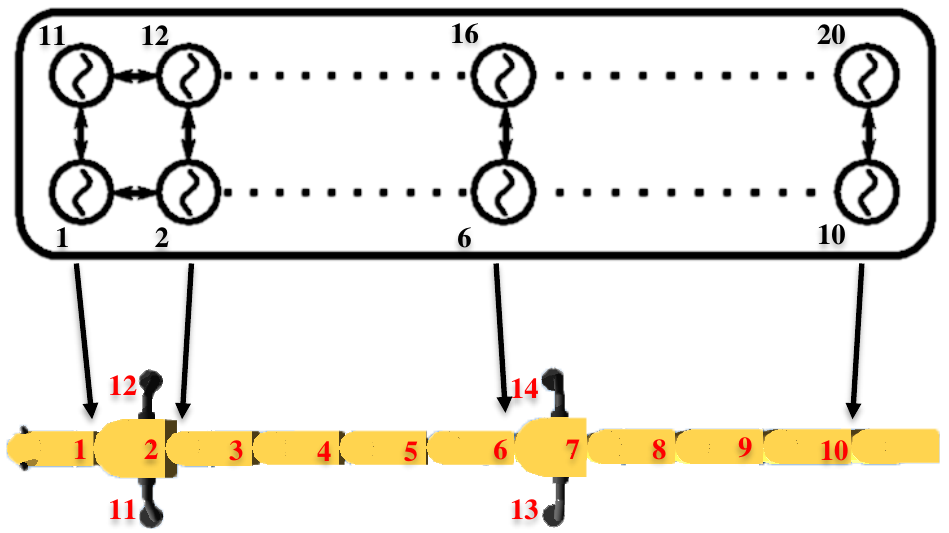
\includegraphics[width=0.5\textwidth]{figures/model_controller.png}
  \caption[Controller model]{A double chain of oscillators controlling the
    robot’s spine.}
  \label{fig:controller-model}
\end{figure}

% \newpage

\subsection*{Code organization}
\label{subsec:code}

\begin{itemize}
\item \corr{\textbf{Webots::worlds::cmc\_salamander.wbt}} - This is the world file which
  describes the world and allows to run the simulation. You can run a simulation
  by running this file with Webots. It also automatically loads the
  pythonController.
\item \corr{\textbf{Webots::controllers::pythonController::pythonController.py}} - The
  main robot controller is implemented in pythonController.py. This file calls
  classes and functions from other files to control the robot and for
  logging. There is also a run\_simulation function which is provided for
  convenience to easily run multiple simulations with different parameters. Note
  that network parameters can be provided here.
\item \corr{\textbf{Webots::controllers::pythonController::cmc\_robot.py}} - Contains the
  SalamanderCMC class, which is used for controlling and logging the robot. Feel
  free to modify this file to extend the logging capabilities. Note that the
  logging makes use of Numpy.savez to save the data.
\item \corr{\textbf{Webots::controllers::pythonController::network.py}} - This file
  contains the different classes and functions for the CPG network and the
  Ordinary Differential Equations (ODEs). You can implement the network
  parameters and the ODEs here. Note that some parameters can be obtained from
  pythonController.py to help you control the values.
\item \corr{\textbf{Webots::controllers::pythonController::solvers.py}} - This
  features fixed time-step solvers which will can are used by network.py for
  solving the ODE at each timestep. Feel free to switch between the Euler and
  the Runge-Kutta methods. \textit{You do not need to modify this files.}
\item \corr{\textbf{Webots::controllers::pythonController::run\_network.py}} - By running
  the script from Python, Webots will be bypassed and you will run the network
  without a physics simulation. Make sure to use this file for question 8a to
  help you with setting up the CPG network equations and parameters and to
  analyse its behaviour. This is useful for debugging purposes and rapid
  controller development since starting the Webots simulation with Python in the
  loop takes a bit of time.
\item \corr{\textbf{Webots::controllers::pythonController::plot\_results.py}} -
  Use this file to load and plot the results from the simulation. This code runs
  with the original pythonController provided.
\item \corr{\textbf{Webots::controllers::pythonController::parse\_args.py}} -
  Used to parse command line arguments for run\_network.py and plot\_results.py
  and determine if plots should be shown or saved directly. \textit{You do not
    need to modify this files.}
\item \corr{\textbf{Webots::controllers::pythonController::save\_figures.py}} -
  Contains the functions to automatically detect and save figures. \textit{You
    do not need to modify this files.}
\end{itemize}

% \newpage

\section*{Prerequisites}

\subsection*{Make sure you have successfully installed Webots by
  following the instructions outlined in Lab 7}

\subsection*{Complete the tutorial and practice examples of Webots as
  outlined in Lab 7}

\subsection*{Open the \fileref{Webots::worlds::cmc\_salamander.wbt} file
  in Webots. This should launch the Salamandra Robotica model in
  simulation world}

\subsection*{Running the simulation}
Now when you run the simulation, the Salamandra Robotica model should
float on the water with no errors in the Webots console dialog. At
this point you can now start to work on implementing your exercises.

\newpage

\section*{Questions}

\subsection*{8a. Implement a double chain of oscillators}
\label{sec:implement-chain}

Salamandra Robotica has 10 joints along its spine. Implement a double
chain (dynamics described in equations \ref{eq:dphase} and
\ref{eq:dr}) of oscillators in a way that lateral oscillator pairs are
assigned to a single joint (see Figure \ref{fig:controller-model}).

\corr{\textit{NOTE} : }No need to implement leg oscillators for this
exercise.

\begin{equation}
  \label{eq:dphase}
  \dot{\phi}_i = 2 \pi f + \sum_j r_j w_{ij} sin(\theta_j - \theta_i - \phi_{ij})
\end{equation}

\begin{equation}
  \label{eq:dr}
  \dot{r}_i = a (R_i - r_i)
\end{equation}

\begin{equation}
  \label{eq:output}
  \dot{q}_i = r_i(1 + cos(\theta_i)) - r_{i+10}(1 + cos(\theta_{i+10}))
\end{equation}

with $ \theta_i $ the oscillator phase, f the frequency, $ w{_ij} $
the coupling weights, $ \phi_{ij} $ the nominal phase lag, $ r_i $ the
oscillator amplitude, $ R_i $ the nominal amplitude, $ a $ the
convergence factor and $ q_i $ the spinal joint angles.

\begin{enumerate}
\item Implement the double chain oscillator model using the functions
  \fileref{network.py::phases\_ode} and
  \fileref{network.py::amplitudes\_ode}. Test your implementation by
  running the network using \fileref{run\_network.py}. For the network
  parameters check lecture slides (pay attention to different number
  of segments). You can set your coupling weight parameters in the
  function \\
  \fileref{network.py::AmplitudeEquations::set\_parameters} and set
  your convergence rates and desired amplitudes in
  \fileref{network.py::PhaseEquations::set\_parameters}
\item Use the output of your CPG network to generate the spinal joint
  angles according to equation \ref{eq:output}. Implement this in the
  function \fileref{network.py::motor\_output}. Verify first in
  Python(\fileref{run\_network.py}) and then in Webots that your code
  works as expected. Use the functions in \fileref{plot\_results.py} to
  report your spinal joint angles $q_i$.
\end{enumerate}


\subsection*{8b. Effects of amplitude and phase lags on swimming performance}
\label{sec:amplitude-phase-performance}

How does phase lag and oscillation amplitude influence the speed and energy? Use
the provided \corr{pythonController.py::run\_simulation()} to run a grid search
to explore the robot behavior for different combinations of amplitudes and phase
lags. Use \corr{plot\_results.py} to load and plot the logged data from the
simulation. Feel free to extend the logging in \corr{cmc\_robot.py} to show
additional measurements if necessary. Include 2D/3D plots showing your grid
search results and discuss them. How do your findings compare to the wavelengths
observed in the salamander? Run the grid search twice, for frequencies of 1Hz
and 2Hz.

\begin{itemize}
\item \textbf{Hint 1:} To use the grid search, check out
  \corr{pythonController.py::run\_simulation()}. This function takes the desired
  parameters as a list and runs the simulation. An example of parameter sweep is
  shown in \corr{pythonController.py::main()} as an example. The function will
  repeatedly run simulations, each time with a different combination of
  parameters from the parameters list. The results are logged as
  simulation\_\#.npz in a specified log folder. After the grid search finishes,
  the simulation will close, you can remove this feature by commenting
  world.simulationQuit(0) in \corr{pythonController.py::main()}.
\item \textbf{Hint 2:} An example how to load and visualise grid search results
  is already implemented in \corr{plot\_results.py::main()}. Pay attention to
  the name of the folder and the log files you are loading. Before starting a
  new grid search, change the name of the logs destination folder where the
  results will be stored. In case a grid search failed, it may be safer to
  delete the previous logs to avoid influencing new results by mistake.
\item \textbf{Hint 3:} Estimate how long it will take to finish the grid
  search. Our suggestion is to choose wisely lower and upper limits of parameter
  vectors and choose a reasonable number of samples. To speed-up a simulation,
  make sure to run Webots in a fast mode.
\item \textbf{Hint 4:} Energy can be estimated by integrating the product of
  instantaneous joint velocities and torques. Feel free to propose your own
  energy metrics, just make sure to include the justification.
\end{itemize}


\subsection*{8c. Amplitude gradient}
\label{sec:amplitude-gradient}

\begin{enumerate}
\item So far we considered constant undulation amplitudes along the body for
  swimming. Implement a linear distribution of amplitudes along the spine,
  parametrized with two parameters: amplitudes of the first (Rhead) and last
  (Rtail) oscillator in the spine (corresponding to the first and last
  motor). To do so, modify the function
  \corr{network.py::AmplitudeEquation::set\_parameters()} such that the input
  variable amplitudes=[Rhead, Rtail] now has the size 2, and within the function
  you interpolate the amplitude gradient between values Rhead and Rtail. Note
  that you can the provide this amplitudes parameter from
  \corr{pythonController.py}.
\item Run a grid search over different values of parameters Rhead and Rtail (use
  the same range for both parameters). How does the amplitude gradient influence
  swimming performance (speed, energy)? Include 3D plots showing your grid
  search results. Do it once, for frequency 1Hz and total phase lag of $2\pi$
  along the spine.
\item How is the salamander moving (with respect to different body amplitudes)?
  How do your findings in 2) compare to body deformations in the salamander?
  Based on your explorations, what could be possible explanations why the
  salamander moves the way it does?
\end{enumerate}


\subsection*{8d. Turning and backwards swimming}
\label{sec:turning-backwards}

\begin{enumerate}
\item How do you need to modulate the CPG network (\corr{network.py}) in order
  to induce turning?  Implement this in the Webots model and plot example GPS
  trajectories and spine angles.
\item How could you let the robot swim backwards? Explain and plot example GPS
  trajectories and spine angles.
\end{enumerate}


% \newpage

\bibliography{lab8}
\label{sec:references}
\bibliographystyle{ieeetr}


% \newpage

% \section*{APPENDIX}
% \label{sec:appendix}

\end{document}

%%% Local Variables:
%%% mode: latex
%%% TeX-master: t
%%% End: